\chapter{Datasets, Training and Evaluation} \lhead{\emph{Datasets, Training and Evaluation}}

In this chapter I will first give a full description of the BOLD inversion teacher forcing algorithm I developed. 
Then I will showcase the datasets on which the models were trained, delve into the specifics of the training routines utilized, 
and discuss the evaluation measures I employed to assess the performance of the trained models.

\section{BOLD inversion teacher forcing}

We recall from section \ref{sec:bold_obs_eq} the BOLD observation equation

\begin{equation}
    \hat{x}_t = O(z_t, r_t) = \boldsymbol{B} \left( (hrf \ast z)_t\right) + \boldsymbol{J}r_t + \epsilon_t.
\end{equation}

To apply the teacher forcing algorithm we need to generate desired target values $d_t$ for the latent states $z_t$ from the ground truth $x_t$

\begin{equation}
    \{d_t\} = O^{-1}(\{x_t, r_t\}) = \left\{\text{Conv}^{-1}\left(\boldsymbol{B}^+ \left(x_t - \boldsymbol{J} r_t \right), hrf \right) \right\}
    \label{eq:bold_inv_naive}
\end{equation}

where $\text{Conv}^{-1}(\cdot, hrf)$ is the deconvolution of data with the $hrf$. Note that we to perform these steps on an entire series $\{x_t\}$
because there is no one-to-one correspondence between a time point $t$ of the unconvoluted and convoluted time series.

The issue with solving the inversion with equation \ref{eq:bold_inv_naive} is that the deconvolution has to be performed in every epoch of training because $B$ is 
learned and doesn't stay constant. The trick is to notice that the same $hrf$ function is applied to all latent space dimensions, hence one can interchange the matrix 
multiplication with $\boldsymbol{B}$ and the convolution step.

Let $Z_{i,t} \in \mathbb{R}^{M \times T}$ be the data matrix of the $M$-dimensional time series of length $T$, $hrf[t] = h_t$ be the hrf vector at an arbitrary
but fixed repeat time and $\boldsymbol{B} = b_{ij} \in \mathbb{R}^{N \times M}$ the observation matrix.

\begin{align}
    \boldsymbol{B} ( hrf \ast Z)_t &= \sum_{i=1}^{M} b_{ij} \sum_{\tau=1}^{T} h_{t - \tau} Z_{j, \tau}  \\
                      &= \sum_{i=1}^{M} \sum_{\tau=1}^{T} h_{t - \tau} b_{ij} Z_{j, \tau} \\
                      &= \sum_{\tau=1}^{T} h_{t - \tau} \sum_{i=1}^{M}  b_{ij} Z_{j, \tau} \\
                      &= \left(hrf \ast (\boldsymbol{B} \cdot Z) \right)_t
\end{align}

Furthermore, we can pull the nuisance variables $r_t$ through the convolution using linearity (see Proposition \ref{prop:conv_properties}). Let $r_t$ be the nuisance variables
and $r_{\text{deconv}_t} = \text{Conv}^{-1}(r_t, hrf)$ the deconvoluted nuisance variables.

\begin{align}
    O(z_t, r_t) &= \boldsymbol{B} \left( (hrf \ast z)_t\right) + \boldsymbol{J}r_t \\
                &= \left(hrf \ast (\boldsymbol{B} \cdot z) \right)_t + \boldsymbol{J}r_t \\
                &= \left(hrf \ast (\boldsymbol{B} \cdot z + \boldsymbol{J} \cdot \text{Conv}^{-1}(r_t, hrf) \right)_t \label{eq:obs_eq_simple}
\end{align}

Equation \ref{eq:obs_eq_simple} now has an inversion, which is computationally much more efficient:

\begin{equation}
    \{d_t\} = O^{-1}(\{x_t, r_t\}) = \{\boldsymbol{B}^{+} \left( \text{Conv}^{-1}(x_t, hrf) - \boldsymbol{J} \cdot \text{Conv}^{-1}(r_t, hrf) \right) \}
\end{equation}

This form lets us compute the deconvoluted time series $\text{Conv}^{-1}(x_t, hrf)$ and \newline $\text{Conv}^{-1}(x_t, hrf)$ once before training. At train time only the 
psuedo-inverse $\boldsymbol{B}^+$ has to be computed and applied as in inversion TF (see Eq. \ref{eq:inversion_tf}).

To compute the deconvolution, first the VISUSHRINK algorithm (see Algorithm \ref{algo:visushrink}) is applied to the time series $\{x_t\}$ to obtain an estimate of the 
noise level $\tilde{\sigma}$ and the denoised signal $\tilde{x_i}$. Then the power spectra of the measured signal, the denoised signal, the noise and the $hrf$
are calculated and used in the Wiener deconvolution filter (see Eq. \ref{eq:wiener_deconv}).
Note that the noise is assumed to be Gaussian white noise, hence the power spectrum is flat $P_i = \tilde{\sigma}^2$.

The Wiener filter is then applied to the observed signal in Fourier space and the result transformed back to the time domain, resulting in the deconvoluted 
time series $\{x_t\}_{deconv}$.

\subsection{Boundary issues and minimum noise level}

There are issues at the boundaries of a signal batch when calculating the deconvolution there. A batch refers to a subset of the dataset. 
Instead of feeding the entire dataset into the model at once in training, the time series data is divided into several batches, 
and the model is trained on each batch one at a time.

The reason is that values from outside the batch were used to calculate 
the values at the edges. The convolution effectively lets information smear out across time. We do however not have access to values from outside the batch and thus
there are typically large errors at the edges of the deconvoluted signal.

Ideally we would cut off the boundaries and only use valid points, i.e. ignore the first and last $\text{length}(hrf)$ points of each batch. In the context of fMRI we are 
however already heavily data constrained with time series of length $\mathcal{O}(10^3)$. In relation to this the length of the $hrf$ impulse is not negligible. For 
example, we have $\text{length}(hrf_{2.0}) = 17$, $\text{length}(hrf_{1.4}) = 27$ and $\text{length}(hrf_{0.8}) = 41$. We can't afford to drop that many data points 
\textit{in each batch}. 

From visual inspection of the deconvolution results, I decided to cut $\frac{1}{4} \text{length}(hrf)$ at the boundaries, as the 
biggest error occur there. The hyperparameters \textbf{cut\_l} and \textbf{cut\_r} set how much of the left and right boundary is cut. The cutoffs of a batch 
are visualized in the figures \ref{fig:high_freq_issues} and \ref{fig:min_conv_noise}.  

In practice, the noise estimation only has a finite precision. For very small noise levels, for example in strongly preprocessed data or even no noise in artificial 
benchmark data, the deconvolution described above encounters numerical issues. The Wiener filter begins to return high frequency artifacts if we let the noise level 
approach $0$ (see figure \ref{fig:high_freq_issues}).  In most experimental cases this should not occur, but noiseless benchmark data and heavily smoothed data 
cause the noise estimation to return values close to $0$.
A hyperparameter \textbf{min\_conv\_noise} is set which is the minimum $\tilde{\sigma}$ the Wiener filter uses to avoid high frequency artifacts. Figures 
\ref{fig:high_freq_issues} and \ref{fig:min_conv_noise} offer a comparison between the simple Wiener filter and one with added minimum noise level. The 
higher frequency oscillations disappear, only the boundaries still contain large deviations from the original signal.

\begin{figure}
    \centering

    \begin{subfigure}[b]{\textwidth}
        \centering
        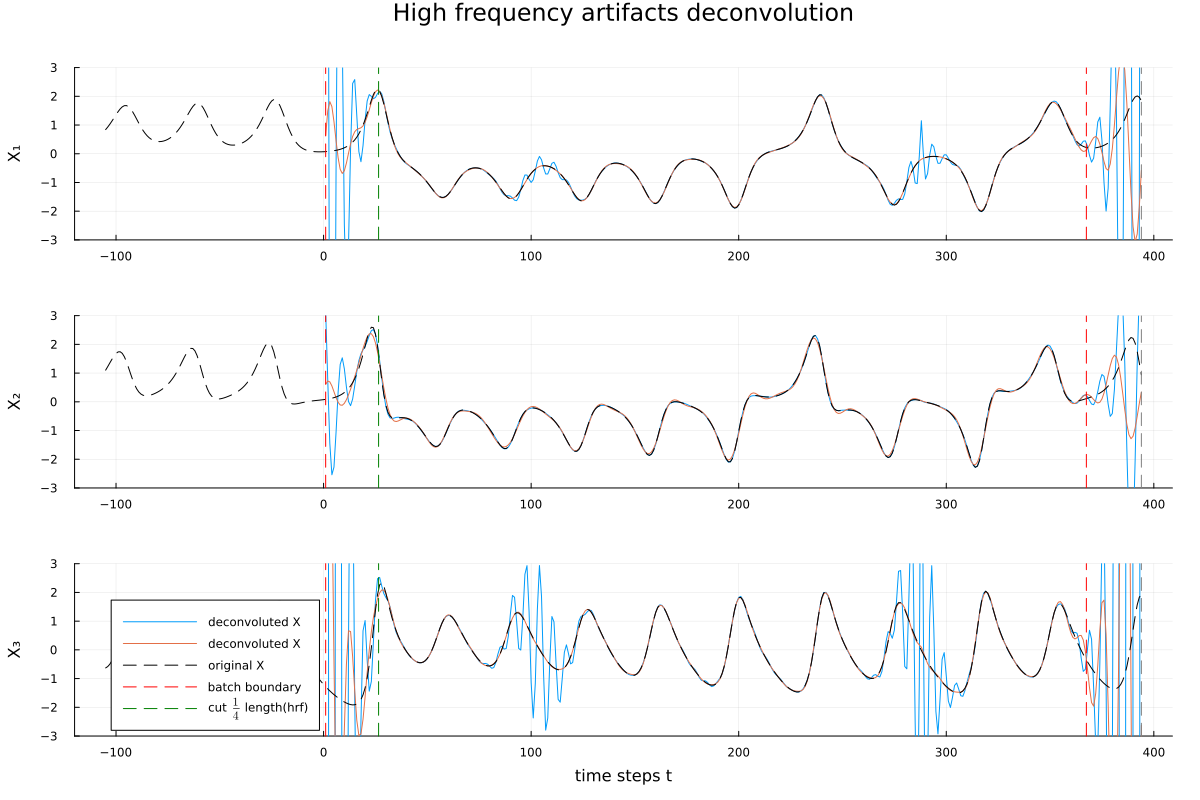
\includegraphics[width=\textwidth]{Images/high_freq_issues.png}
        \caption{Deconvolution of a Lorenz63 time series with no noise component. Deconvolution returns high frequency artifacts both at the 
                 boundaries and throughout the signal.}
        \label{fig:high_freq_issues}
    \end{subfigure}

    \begin{subfigure}[b]{\textwidth}
        \centering
        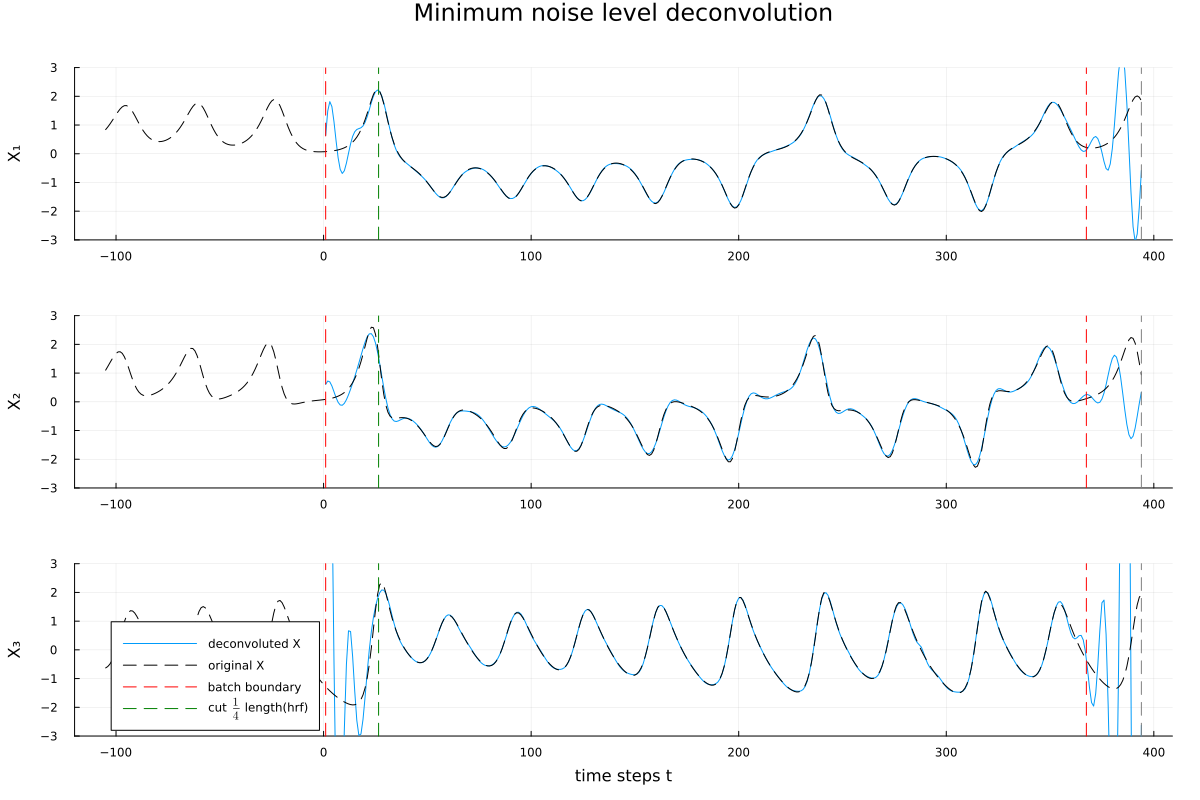
\includegraphics[width=\textwidth]{Images/min_conv_noise.png}
        \caption{Deconvolution of a Lorenz63 time series with no noise component, but minimum noise level set. High frequency artifacts are much smaller and only 
                appear close to the boundaries within the $\frac{1}{4}\text{length}(hrf)$ cutoffs.}
        \label{fig:min_conv_noise}
    \end{subfigure}

       \caption[Deconvolution issues exemplified by a Lorenz63 time series]{Deconvolution issues exemplified by a Lorenz time series}
       \label{fig:three graphs}
\end{figure}

A full description of the deconvolution algorithm which was finally implemented and used for the experiments is given in Algorithm \ref{algo:deconv_full}.

\begin{algorithm}[htb]

    \hspace*{\algorithmicindent} \textbf{Input:} time series data $x_i$ of length $N$; analyzing wavelet $\psi$;\\ \hspace*{\algorithmicindent} \phantom{Input:  } minimum noise level $\tilde{\sigma}_{min}$;
    boundary cutoffs cut\_l, cut\_r;  \\ 
    \begin{enumerate}
        \item Apply the VISUSHRINK algorithm (see Algorithm \ref{algo:visushrink}) to the time series $\{x_t\}$ to obtain an estimate of the 
        noise level $\tilde{\sigma}$ and the denoised signal $\tilde{x_i}$

        \item \textbf{If} $\tilde{\sigma} < \tilde{\sigma}_{min}$ \textbf{then} Set $\tilde{\sigma} := \tilde{\sigma}_{min}$

        \item Compute the Fourier transform of the $hrf$ and the power spectra of the observed signal, the denoised signal 
              and the noise. The noise is assumed to be Gaussian white noise, hence the power spectrum is flat $P_i = \tilde{\sigma}^2$.

        \item Compute the Wiener filter (see Eq. \ref{eq:wiener_deconv}). The power spectrum of the denoised signal is used as input
              $S(k)$, the power spectrum of the original signal in Eq. \ref{eq:wiener_deconv}.
        
        \item Apply the Wiener deconvolution filter (see Eq. \ref{eq:wiener_filter_fourier}) to measured signal in Fourier space
        
        \item Transform the result back to the time domain to obtain $\{x_t\}_{deconv}$.
        
        \item Edges of signal are set to NaN as they contain artifacts and can't be used. \newline
              $x \left[\text{begin}:\text{begin} + \text{cut\_l} \right] = \text{NaN}$, $x \left[\text{end}-\text{cut\_r}:\text{end}\right] = \text{NaN}$
    \end{enumerate}
    \hspace*{\algorithmicindent} \textbf{Output:} estimate of the deconvoluted signal $\{x_t\}_{deconv}$;\\ 
    \caption{The full deconvolution Algorithm}
    \label{algo:deconv_full}
\end{algorithm}

\section{Evaluation metrics} \label{sec:eval_metrics}

There is a major problem when evaluating the performance of models on chaotic time series. It can easily be seen when remembering the concept of Lyapunov exponents 
(c.f. \ref{sec:lya_exp}). If the maximum Lyapunov exponent of a system is larger than $0$, $\lambda_{\max} > 0$, which is a necessary condition of chaos, nearby trajectories
diverge exponentially quickly. This limits the applicability of $n$-step ahead prediction errors, as even small numerical errors will lead to exponentially growing 
prediction errors.

We therefore need different tools to evaluate the performance of models trained on chaotic time series which depend on properties invariant to the initial conditions.
In this work, I will use two measures that have been established (\cite{mikhaeil2022difficulty}) to robustly evaluate the performance on chaotic data. 
The first is a state space measure that focuses on geometric properties of the time series and the other is based on the power spectrum. 

\subsection{State Space Distance \texorpdfstring{$D_{stsp}$}{Lg}} \label{sec:d_stsp}

The general idea of this measure was introduced in \cite{koppe2019identifying}. 
Given an observed $N$-dimensional time series $\{x_t\}$ of length $T$ and a
time series $\{\hat{x}_t\}$ with the same dimension/length generated by a model aiming to reconstruct the dynamical system underlying $\{x_t\}$, $D_{stsp}$ measures
the geometrical overlap of orbits in state space.

For low dimensional systems $N \leq 6$ the state space is separated into $k^N$ bins where $k$ is the number of bins per dimension. Each bin is given a label $i$ and 
the number of points $n_i$ of the time series is within that bin is measured. This gives us the relative frequency of that bin

\begin{equation}
    p_i = \frac{n_i}{T}.
    \label{eq:rel_freq}
\end{equation}

Combining these frequencies across all bins in space results in a probability distribution which approximates the state space distribution of the underlying dynamical system.
Then the Kullback-Leibler-Divergence (KLD) of the empirical distributions can be calculated to give a measure of the overlap of both systems in state space:

\begin{equation}
    D_{stsp} = \sum_{i=1}^{k^N} p_i \log \left(\frac{p_i}{q_i}\right)
\end{equation}

where $p_i$ are the relative frequencies of the measured time series and $q_i$ are the relative frequencies of the generated time series. Note that KLD is not a metric in 
the mathematical sense, but instead it is a divergence which establishes the separation of probability distributions.

The complexity of this binning approach scales exponentially with the observation dimension $N$ and thus becomes intractable with growing $N$. To compute $D_{stsp}$ in higher 
dimensional systems, \cite{brenner2022tractable} use a Gaussian mixture model with centers (means) $x_t$ and diagonal covariance 
$\boldsymbol{\Sigma}=\text{diag}(\sigma^2, \cdots, \sigma^2)$ where $\sigma$ is a hyperparameter. The GMMs of a time series are given by 

\begin{equation}
    f(y) = \frac{1}{T} \sum_{t=1}^{T} \mathcal{N}(y;x_t,\boldsymbol{\Sigma}).
\end{equation}

Following \cite{hershey2007approximating}, the KLD of the two GMMS can be computed using a Monte-Carlo sampling approach 

\begin{equation}
    D_{stsp} \approx \frac{1}{K} \sum_{i=1}^{K} \log \left(\frac{f_{obs}(y_{i})}{f_{gen}(y_{i})}\right) 
             = \frac{1}{K} \sum_{i=1}^{K} \log \Bigg ( \frac{1/T \sum_{t=1}^{T} \mathcal{N}\left( y_i;x_t;\boldsymbol{\Sigma}\right)}{1/T \sum_{t=1}^{T} \mathcal{N}\left(y_i;\hat{x}_t;\boldsymbol{\Sigma}\right)}\Bigg )
\end{equation}

where $K$ is the number of samples drawn, $f_{obs}$ is the distribution of the observed time series and $f_{gen}$ is the distribution of the generated time series.
This approach can be interpreted as an adaptive binning approach only considering bins with points in them. While the two measures correlate strongly in low dimensions,
it is difficult to validate the GMM approach in high dimensional systems.

\subsection{Power Spectrum Error \texorpdfstring{$D_{PSE}$}{Lg}} \label{sec:d_pse}

The previously introduced state space measures discards all temporal structure of the data. To include temporal information in the model evaluation I will also use the 
power spectra of the observed and generated time series. For each dimension $i \in [\![0, N]\!]$ the scalar time series $\{x^{(i)}_t\}$ can be used to 
calculate a power spectrum density (PSD) $\{S^{(i)}_k\}$. The components are calculated from the Fourier transform of $\{x^{(i)}_t\}$.

\begin{equation}
    S_k^{(i)} = \frac{|\widehat{x}^{(i)}_k|}{T} = \frac{| \mathscr{F}\{x^{(i)}_t\}_k |}{T}
\end{equation}

To evaluate the agreement of power spectra the Hellinger Distance (HD) is used as suggested by \cite{mikhaeil2022difficulty}. Since HD is a probability measure 
the computed power spectra have to be normalized:

\begin{equation}
    \bar{S}^{(i)}_k = \frac{S^{(i)}_k}{\sum_{j=1}^{T}S^{(i)}_j}
\end{equation}

The Hellinger Distance is then calculated as follows using the power spectra of the observed time series  $p^{(i)}_k = \bar{S}^{(i)}_k(\{x^{(i)}_t\})$ and 
the generated time series $q^{(i)}_k = \bar{S}^{(i)}_k (\{\hat{x}^{(i)}_t\})$

\begin{equation}
    D_H^{(i)} = \sqrt{1 - \sum_{k = 1}^{T}\sqrt{p^{(i)}_i q^{(i)}_i}}
    \label{eq:hellinger_dist}
\end{equation}

The power spectrum error is computed by averaging the Hellinger Distances across all $N$ dimensions of the observed system.

\begin{equation}
    D_{PSE} = \frac{1}{N} \sum_{i = 1}^{N} D_H^{(i)}
    \label{eq:d_pse}
\end{equation}

Before any computations the power spectra typically have to be smoothed with a Gaussian kernel with width $\sigma$ to reduce the noise. This is another 
hyperparameter that has to be chosen to evaluate a model.

\section{Datasets}

The methods developed in this thesis are applied to both synthetic benchmark datasets and real world datasets. As benchmark system I used the Lorenz63 system which 
was convoluted different $hrf$ functions and obfuscated with different noise levels. The advantage of such a benchmark system is that the latent, 
(unconvoluted and noiseless) trajectories of the system are known. This allows us to evaluate the model outputs both in the latent space and the observation or 
measurement space. As real fMRI data I used the publicly available dataset by the MPI Leipzig (\cite{babayan2019mind}), which contains task-free 
resting-state fMRI (rs-fMRI) of 227 healthy participants together with range of physiological measurements, cognitive tests and emotion/personality tests.

\subsection{Lorenz63 System}

The Lorenz63 introduced in \cite{lorenz1963deterministic} was designed to describe atmospheric convection based on three observables. A two-dimensional fluid layer is 
uniformly warmed from below and cooled from above. It is a continuous dynamical system given by the following set of differential equations:

\begin{align}
    \frac{dx_1}{dt} &= \sigma (x_2 - x_1) \\
    \frac{dx_2}{dt} &= x_1 (\rho - x_3) - x_2 \\
    \frac{dx_3}{dt} &= x_1 x_2 - \beta x_3  
\end{align}

where $x_1$ is proportional to the rate of convection, $x_2$ to the horizontal temperature variation and $x_3$ to the vertical temperature variation. The constants 
are $\alpha$, $\rho$ and $\beta$ are system parameters proportional to the Prandt number, Rayleigh number and certain physical dimensions of the fluid-layer. To produce 
chaoticity the following parameters are typically used: $\sigma=10$, $\rho=28$ and $\beta = \frac{8}{3}$. These settings produce the so-called "butterfly attractor" 
characteristic of the Lorenz system. Example trajectories are shown in Figure \ref{fig:lorenz_system}.

\begin{figure}
    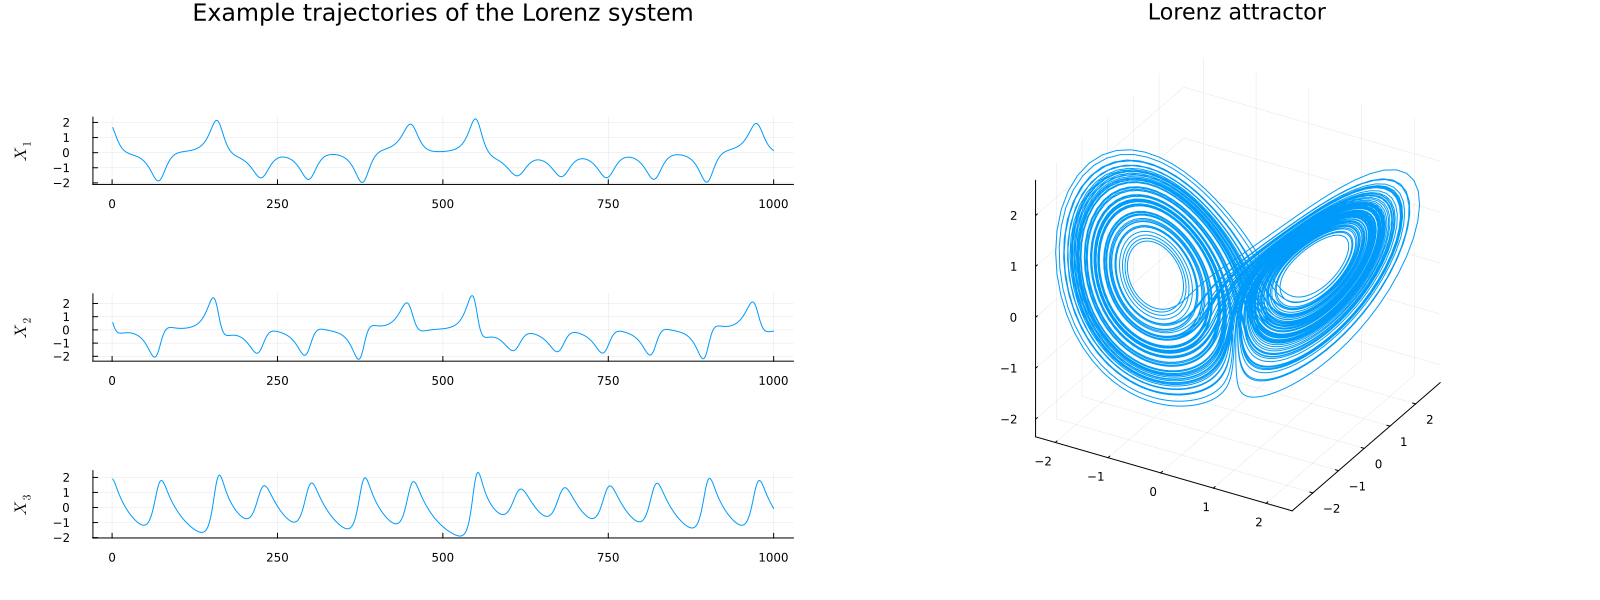
\includegraphics[width=\textwidth]{Images/lorenz_system.png}
    \caption[Simulated data of the Lorenz System]{\textbf{Simulated data of the Lorenz System: } Example trajectories with 1000 time steps. 
    Lorenz attractor with characteristic butterfly wing shape in 3D state space}
    \label{fig:lorenz_system}
\end{figure}

\subsection{LEMON Dataset}

The LEMON ("Leipzig Study for Mind-Body-Emotion Interactions") dataset is a publicly available dataset published by the MPI Leipzig \cite{babayan2019mind}. 
It consists of 227 healthy participants divided into a young ($N=153$) and an elderly group ($N=74$). Each of the participants completed a battery of tests for
physiological assessment, including 6 cognitive tests and 18 emotion- and personality-related questionnaires, a 62-channel EEG experiment at rest and 
a task-free resting-state fMRI scan while further physiological measures were continuously acquired (blood-pressure, heart-rate, pulse, respiration). The full details of 
the dataset and the data acquisition can be found in \cite{babayan2019mind}.

In this work I will solely focus on the rs-fMRI data and not use the other data modalities for training the models. Utilizing the preprocessed fMRI data in the dataset,
time series from 16 regions of interest (ROIs) were extracted. These time series were subsequently smoothed, band-pass filtered and standardized to have a mean of 0 and
a standard deviation of 1. This routine was copied from \cite{koppe2019identifying} which provides more details on the preprocessing.
Example trajectories are shown in figure \ref{fig:fmri_example}.

\begin{figure}
    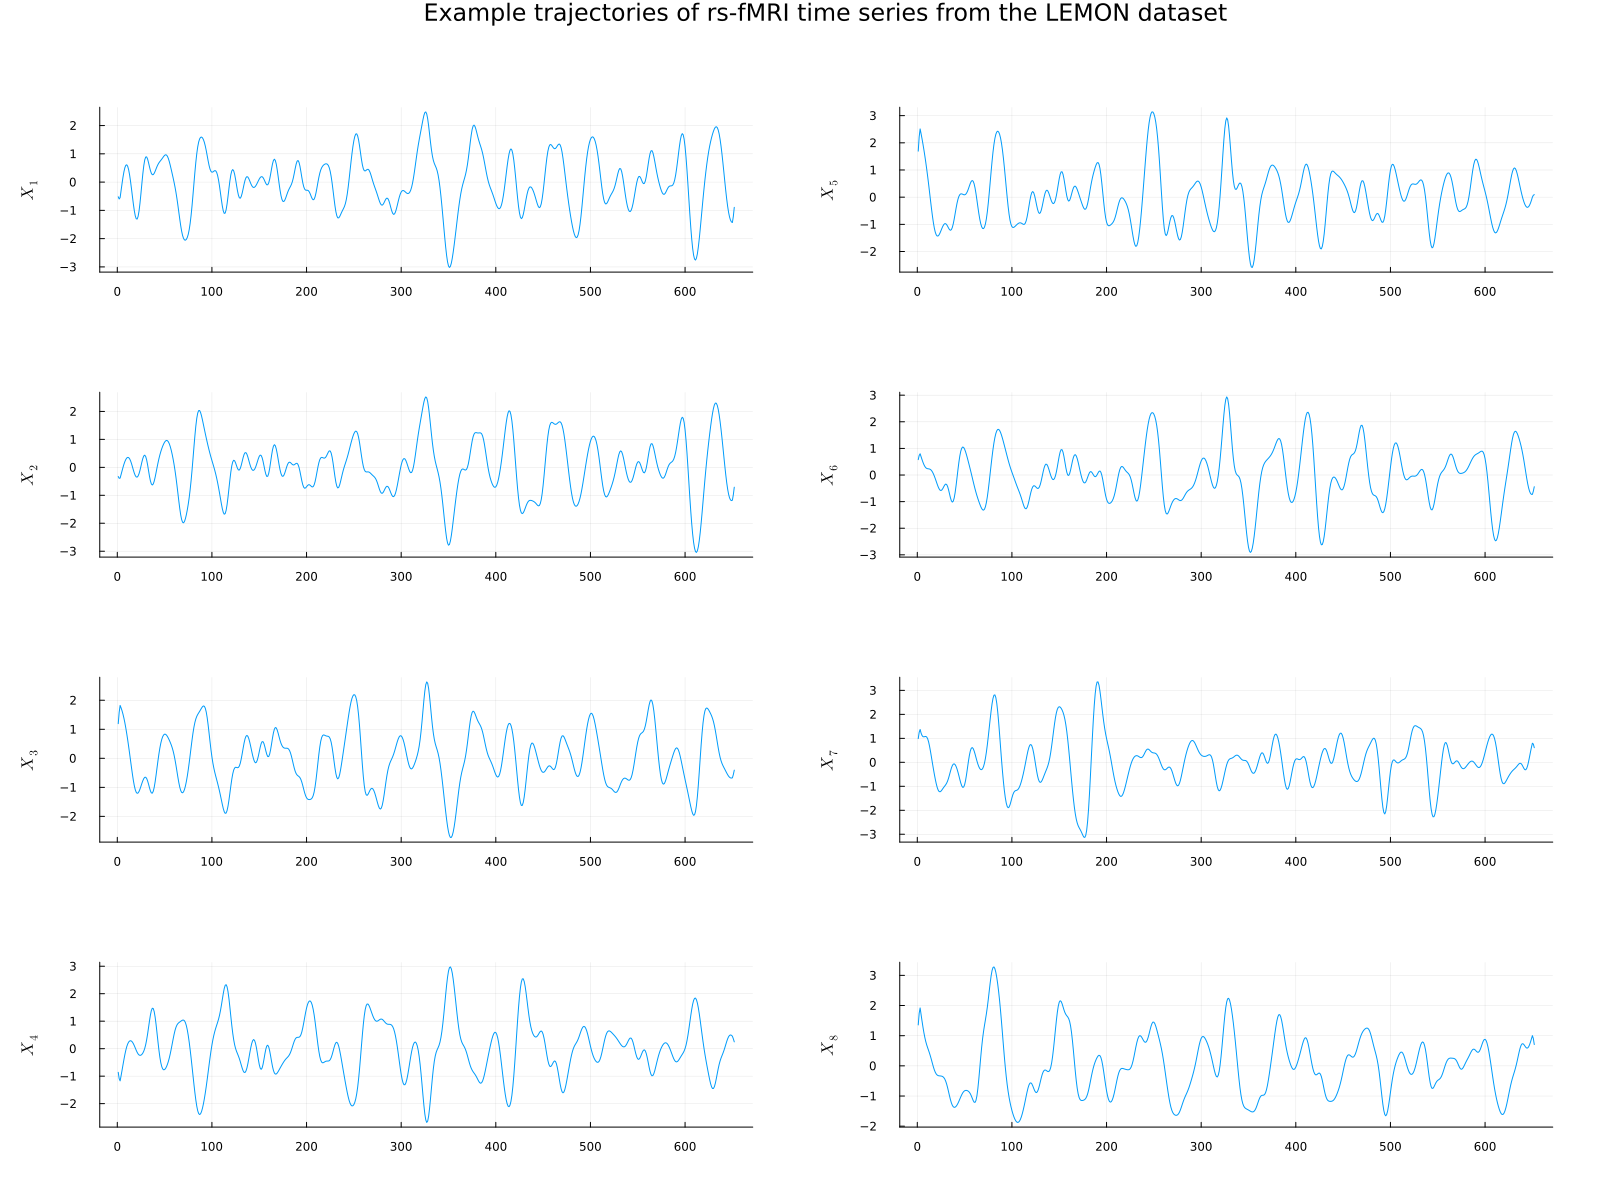
\includegraphics[width=\textwidth]{Images/fmri_example_traj.png}
    \caption[Example trajectories of fMRI time series]{First 8 dimensions of a resting state fMRI time series from the LEMON dataset}
    \label{fig:fmri_example}

\end{figure}

\FloatBarrier
\section{Experimental Setup: Benchmarking on Lorenz63 data}

To benchmark the BOLD inversion algorithm and provide a proof of concept I used the following two setups:

\subsection{Benchmarking on data without noise}\label{sec:noiseless_lorenz}
\begin{enumerate}
    \item I simulated the Lorenz63 system in the chaotic regime to create a dataset containing $10^5$ time steps.
    
    \item I trained a shallowPLRNN model with 5000 epochs on this dataset using weak identity teacher forcing and the identity mapping as observation model.

    \item Using the model training in the previous step I created 4 datasets, each containing 100 trajectories of length $1.1 \cdot 10^6$ drawn from the model. The initial conditions
          were slightly perturbed with Gaussian white noise ($\mu=0, \sigma=1$) and the first $10^5$ time steps discarded to ensure the model has reached its limiting set.

          In the linear case I did not further modify the data. In the other cases I convoluted the data with an $hrf_{1.2}$, an $hrf_{0.5}$ and an $hrf_{0.2}$ respectively.
          These datasets were split 50:50\% as training and test set for the benchmark.

    \item To benchmark, I trained 100 models with the linear identity mapping on each of the datasets. Next, I trained 100 models with BOLD observation model on each dataset.
          For the impulse response I used the same $hrf$ used to generate the dataset. In the case of the linear data without any convolution I used the $hrf_{1.2}$. 
          Each model was trained for 1000 epochs.

    \item After every 25 training epochs a trajectory is generated by the model and the state space distance $D_{stsp}$ and the power spectrum error $D_{PSE}$ are calculated
          so that we have access to the evolution of the Loss, $D_{stsp}$ and $D_{PSE}$ across training when evaluating the benchmark.
\end{enumerate}

A visualization of these convoluted datasets is shown in figure \ref{fig:lorenz_conv}. The complete hyperparameter settings of the training, 
such as the used optimizer, batch size etc. is given in the appendix, table \ref{tab:args lorenz runs}.

\begin{figure}
    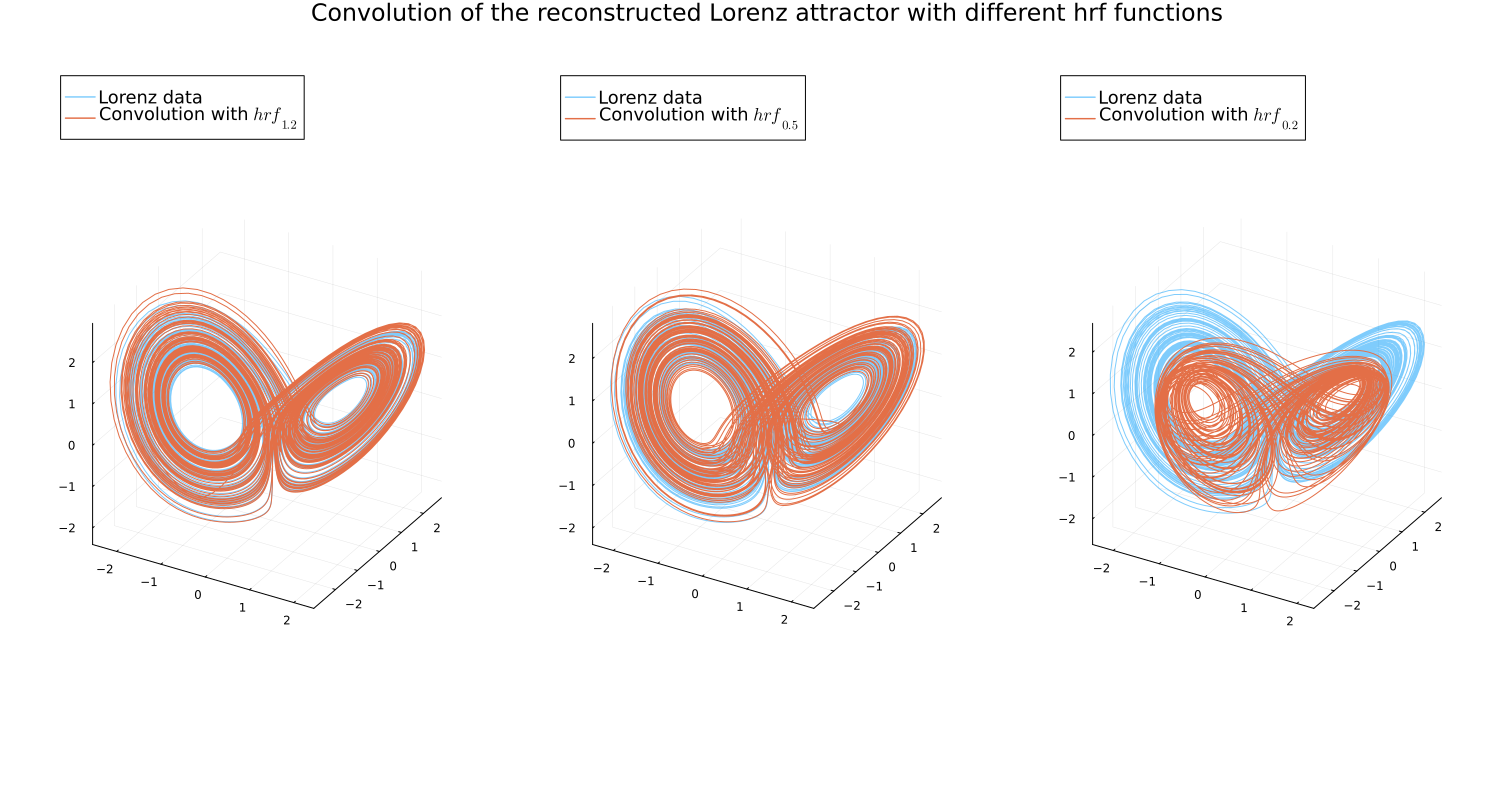
\includegraphics[width=\textwidth]{Images/lorenz_conv.png}
    \caption[Convolution of the reconstructed Lorenz attractor with different $hrf$-functions]
    {Convolution of the reconstructed Lorenz attractor with different $hrf$-functions}
    \label{fig:lorenz_conv}

\end{figure}

\subsection{Benchmarking on data with noise}\label{sec:noisy_lorenz}
\begin{enumerate}
    \item I simulated the Lorenz63 system in the chaotic regime to create a dataset containing $10^5$ time steps

    \item I trained a shallowPLRNN model with 5000 epochs on this dataset using weak identity teacher forcing and the identity mapping as observation model.
    
    \item Using the model trained in the previous step I created 8 datasets, each containing 100 trajectories of length $1.1 \cdot 10^5$ drawn from the model. The initial conditions
          were slightly perturbed with Gaussian white noise ($\mu=0, \sigma=1$) and the first $10^4$ time steps discarded to ensure the model has reached its limiting set.

          In the linear case I added Gaussian white noise to two datasets, once with $\sigma=0.01$ and once with $\sigma=0.1$. For the others I convoluted two datasets 
          each with an $hrf_{1.2}$, an $hrf_{0.5}$ and an $hrf_{0.2}$ respectively. Then I again added Gaussian white noise to the datasets, 
          once with $\sigma=0.01$ and once with $\sigma=0.1$. These datasets were split 50:50\% as training and validation set for the benchmark.

    \item To benchmark, I trained 100 models with the BOLD observation model on each dataset with the respective impulse response used to create the dataset. I also trained 
          with all three impulse responses, $hrf_{1.2}$,  $hrf_{0.5}$ and $hrf_{0.2}$ on the unconvoluted datasets.

    \item After every 25 training epochs a trajectory is generated by the model and the state space distance $D_{stsp}$ and the power spectrum error $D_{PSE}$ are calculated
          so that we have access to the evolution of the Loss, $D_{stsp}$ and $D_{PSE}$ across training when evaluating the benchmark. The generated trajectories have the same
          length as the trajectory from the test set, $5\cdot 10^4$ in this case.
\end{enumerate}

\begin{figure}
    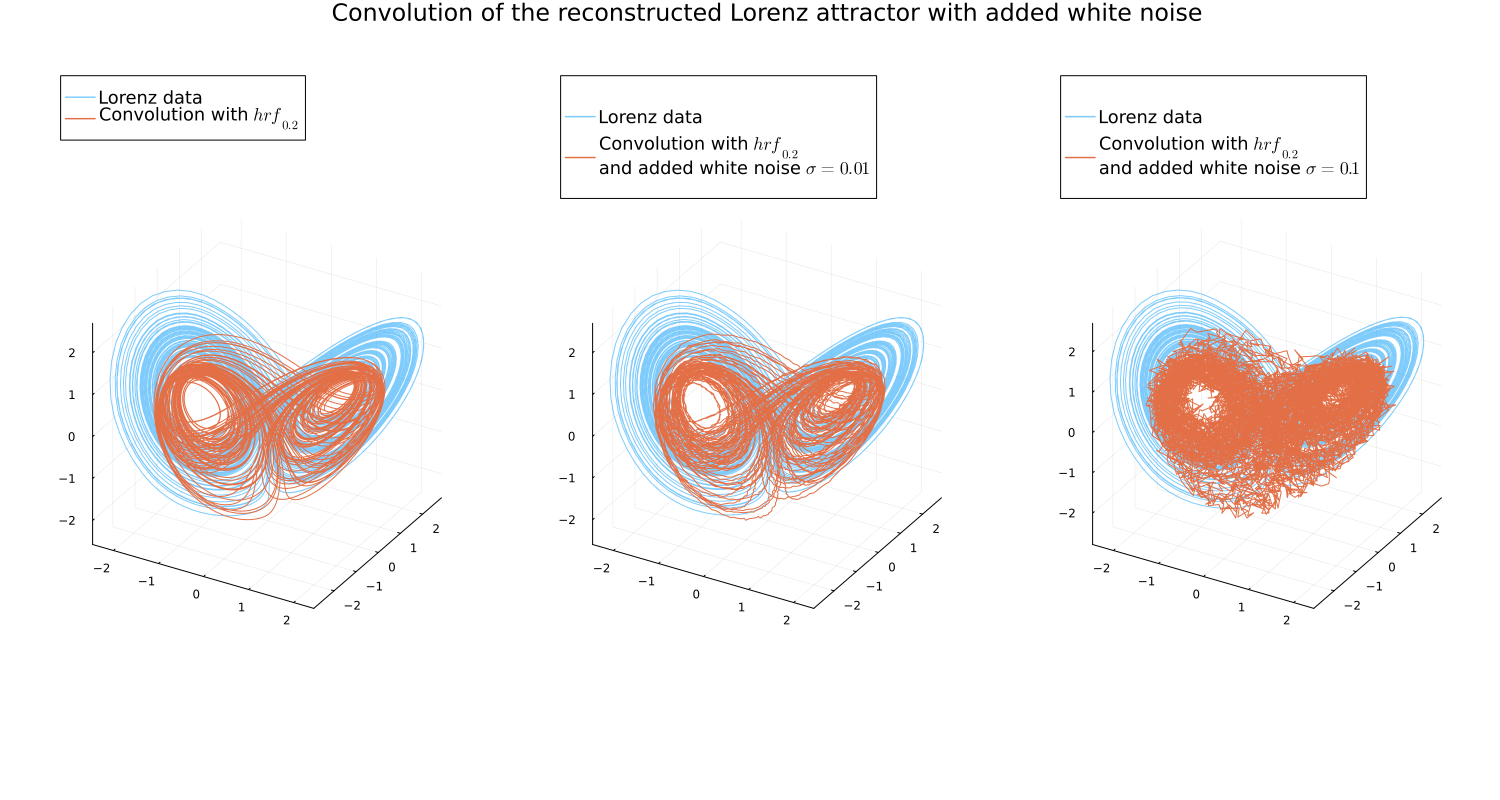
\includegraphics[width=\textwidth]{Images/lorenz_conv_noise.png}
    \caption[Example of noisy convoluted Lorenz attractor]{Example of noisy convoluted Lorenz attractor}
    \label{fig:lorenz_conv_noise}
\end{figure}

An example of these noisy trajectories is shown in figure \ref{fig:lorenz_conv_noise}. Again, the list of hyperparameters are given in table \ref{tab:args lorenz runs}.

\section{Experimental Setup: Filtering LEMON datasets} \label{sec:filter_lemon}

When investigation the time series of the LEMON datasets I noticed the training results varied greatly between participants. Evaluating models trained with the same hyperparameters
on different participants returned different very large differences on the validation set, which was chosen as the last 25\% of the data points.

\begin{figure}
    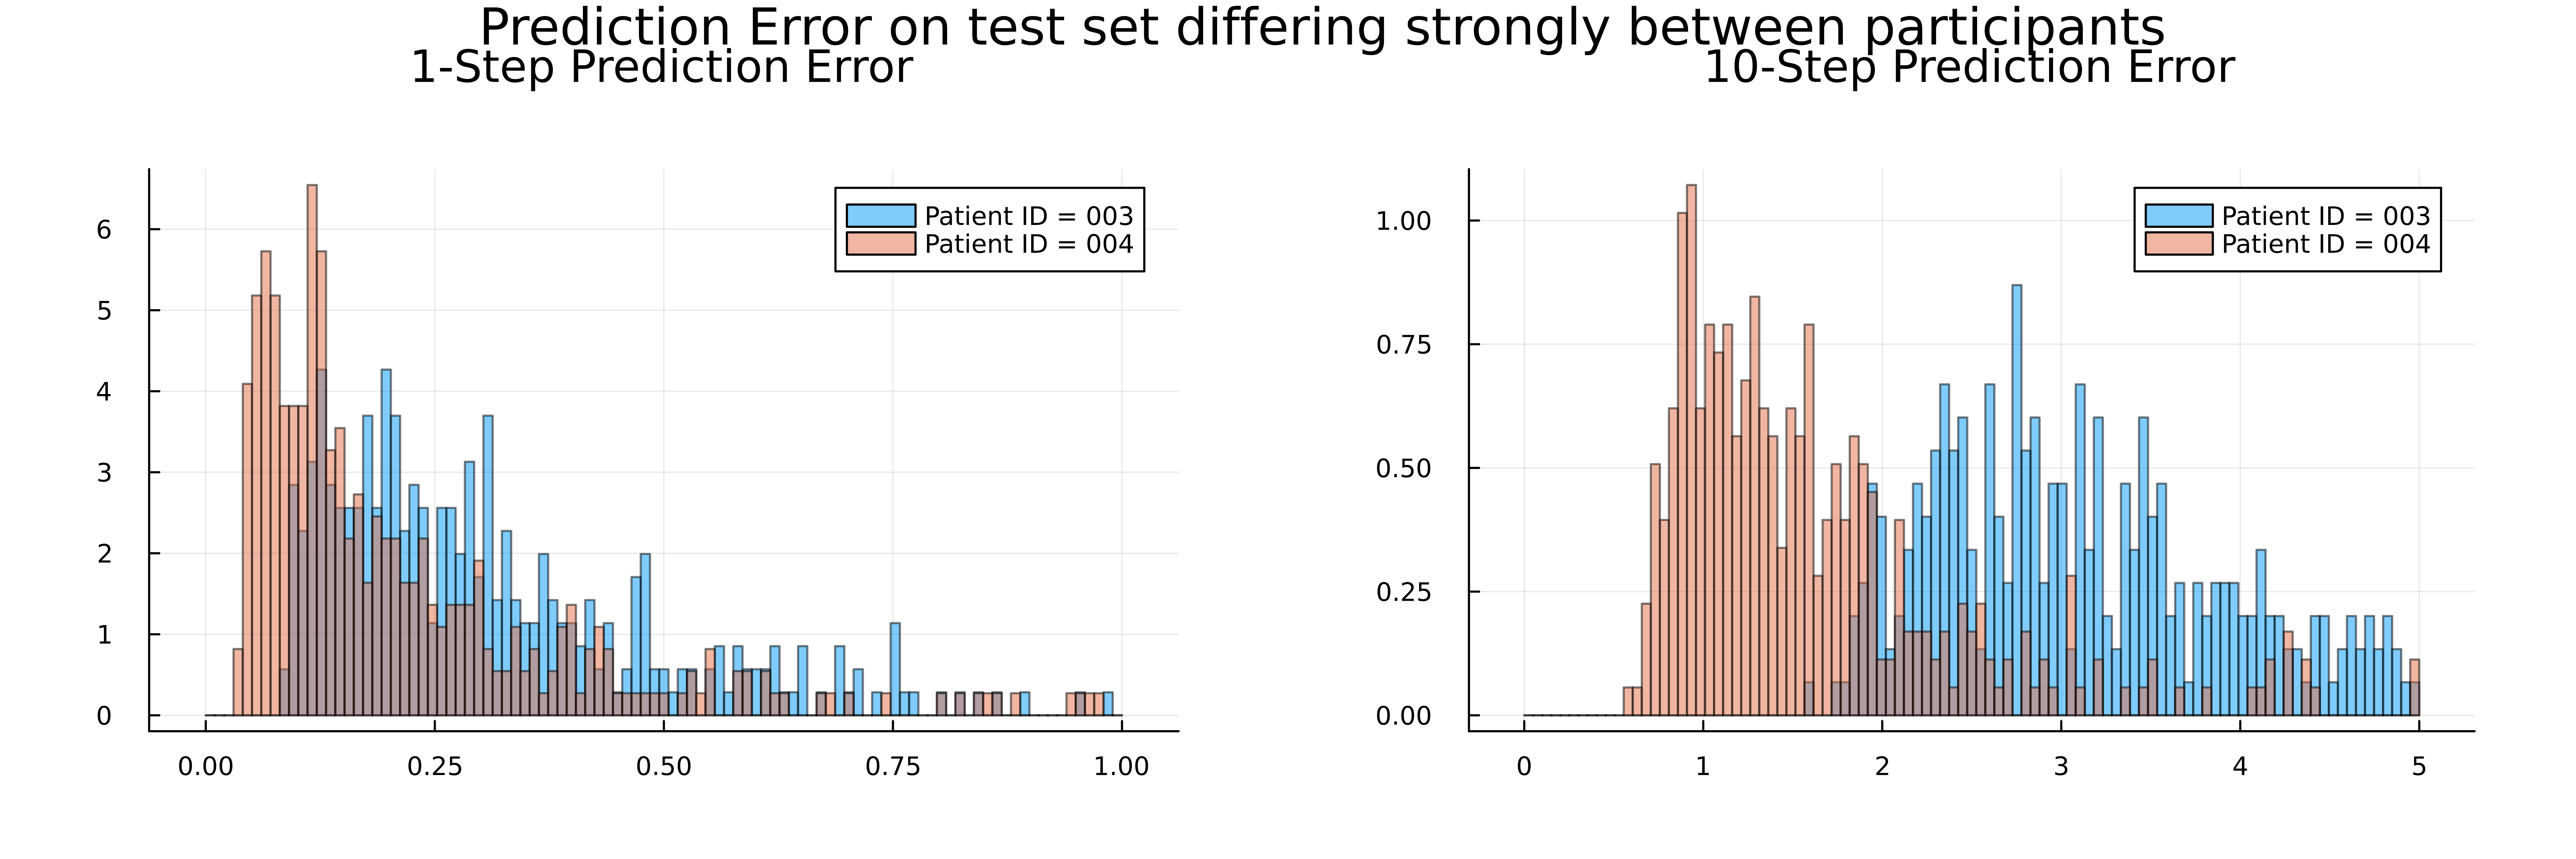
\includegraphics[width=\textwidth]{Images/high_var_patient_pe_comparison.png}
    \caption[Prediction Error on test set differing strongly between participants]
    {\textbf{Prediction Error on test set differing strongly between participants: } Distribution of prediction errors on two different participants ($N=398$). The prediction capability of
    the models trained on participant 003 (\textit{blue}) is significantly worse than those trained on participant 004 (\textit{orange}). Set of hyperparameters for training did not 
    differ between participants.}
    \label{fig:high_var_patient_pe_comparison}
\end{figure}

Following a suggestion by Alena Brändle I looked at the moving averages and moving variances of the time series to see how they evolve with time. Given a window size $w$,
an $N$ dimensional time series $\{x_t\}$ and a dimension $i \in [\![0, N]\!]$  the simple moving average ($SMA$) and variance ($SMV$) are calculated as follows

\begin{align}
    SMA_k^{(i)} &= \frac{1}{w} \sum_{t=k}^{k+w} x_t^{(i)} \\
    SMV_k^{(i)} &= \frac{1}{w} \sum_{t=k}^{k+w} (x_t^{(i)} - SMA_k)^2
\end{align}

Then we average over all dimensions:

\begin{align}
    SMA_k = \frac{1}{N} \sum_{i=1}^{N} SMA_k^{(i)} \\
    SMV_k = \frac{1}{N} \sum_{i=1}^{N} SMV_k^{(i)}
\end{align}

This results in two scalar time series that can easily be visualized and give us an intuition how the underlying fMRI time series evolves. This does however introduce a 
hyperparameter, the window size $w$. There is no simple criterion to decide on a window size. A large window will oversmooth the data while a small window will result 
many noise artifacts remaining. I chose a window size $w=40$ are is delivered good results upon visual inspection.
In figure \ref{fig:sma_smv_example} the SMA and SMV for different participants are shown. Clearly, the variance is not constant but varies greatly 
throughout time. Constant variance, however, is a necessary condition for stationarity. 

\begin{figure}
    \includegraphics[width=\textwidth]{Images/example_sma_smv.png}
    \caption[Simple moving average and variance of different participants]{\textbf{Simple moving average and variance of different participants: } Example of SMA and SMV plotted
    for the first 4 participants in the LEMON dataset (participant 1 is not in the data). Window size $w=40$, the mean of the SMV is subtracted to center it around 
    $0$ and improve presentation.}
    \label{fig:sma_smv_example}
\end{figure}

To quantify the relationship between variance and time I calculated the correlation between them for each participant's SMV. The result is shown in the figure \ref{fig:smv_cor_histo}.

\begin{figure}
    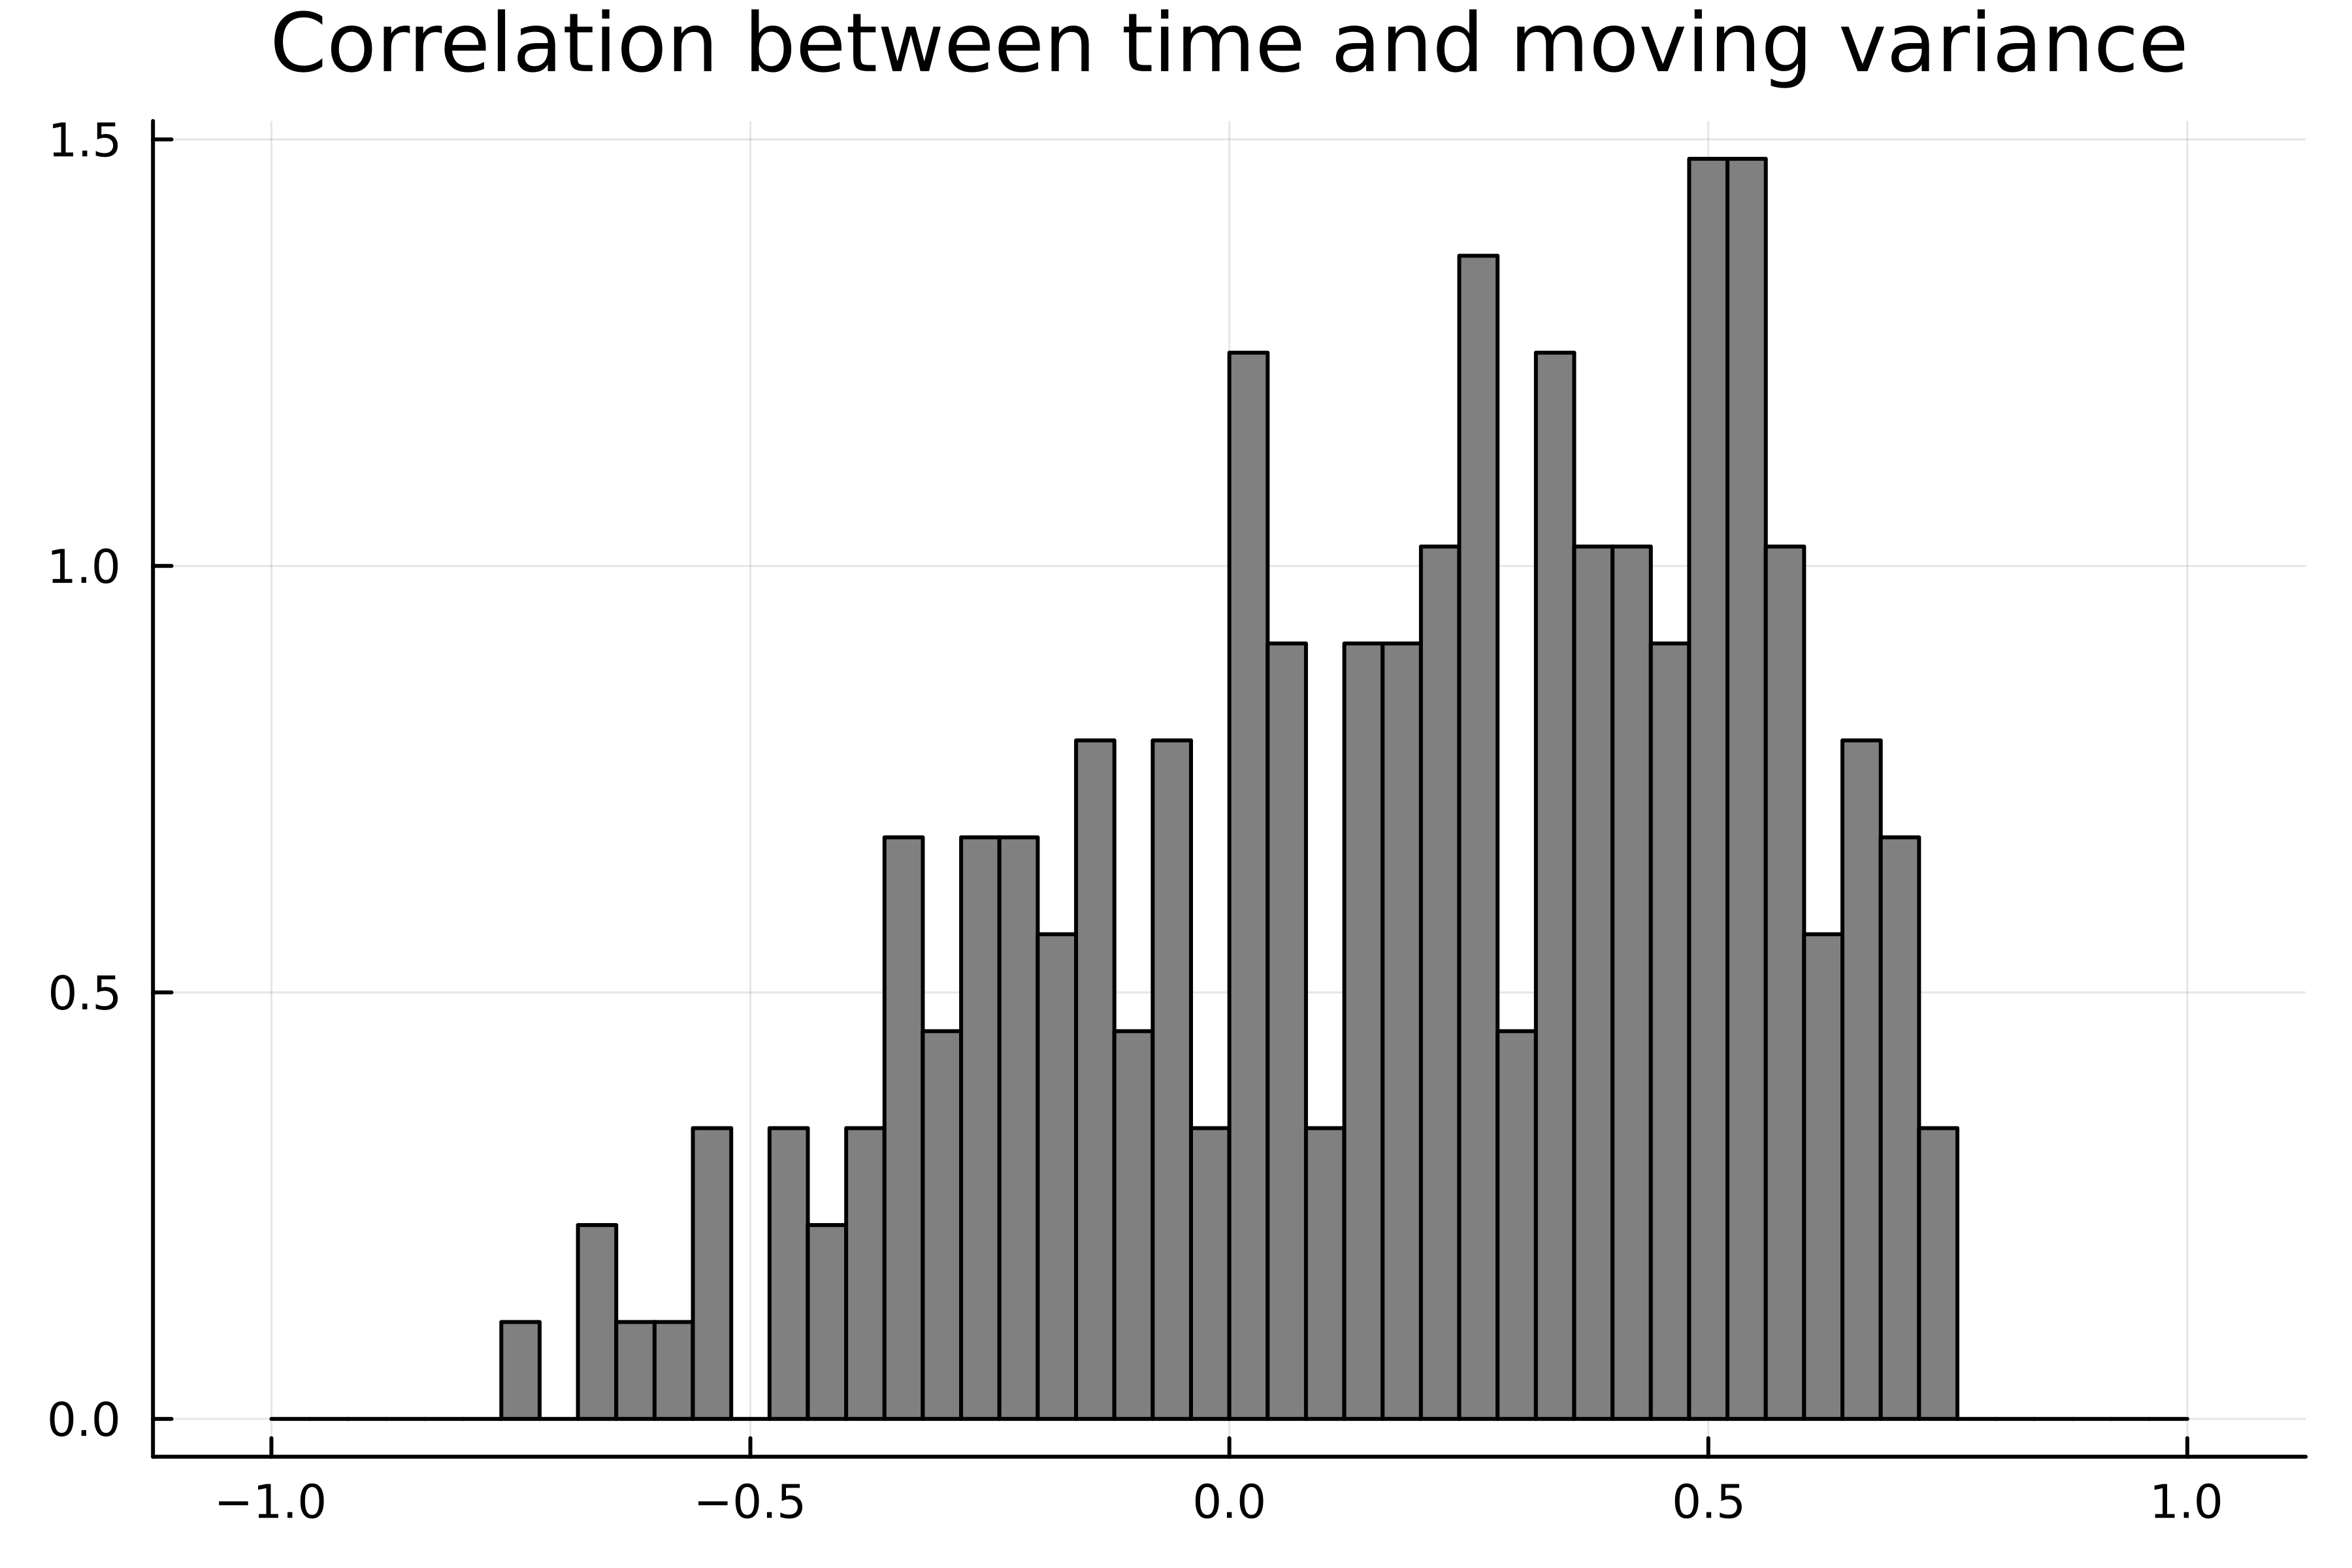
\includegraphics[width=\textwidth]{Images/smv_cor_histo.png}
    \caption[Correlation between time and moving variance]{\textbf{Correlation between time and moving variance: } Normalized histogram of the Pearson correlation between time 
    and moving variance of the time series in the LEMON dataset. Window size $w=40$, bin size $b=0.04$.}
    \label{fig:smv_cor_histo}
\end{figure}

I chose to filter the LEMON dataset by only including the participants with a correlation of less than $0.16$ (the 8 center bins around 0 in the histogram). This leaves 
51 participants for the further experiments in this thesis. The time series are always split 75:25\% into training and test set and the test set is always the 
last 25\% of time points.

\section{Evaluation Setup: Choosing hyperparameters for \texorpdfstring{$D_{stsp}$}{ Lg} and \texorpdfstring{$D_{PSE}$}{Lg}} \label{sec:eval_metrics_param}

As mentioned in the introduction of the metrics $D_{stsp}$ and $D_{PSE}$ in sections \ref{sec:d_stsp} and \ref{sec:d_pse}, they each require a hyperparameter. 
In the case of $D_{stsp}$ this is the scaling parameter of the GMM, in the case of $D_{PSE}$ this is the smoothing $\sigma$ Gaussian kernel used to smooth the 
power spectra. In \cite{brenner2022tractable} these parameters are set to 1.0 and 20 respectively. Unlike the datasets used in \cite{brenner2022tractable}, 
the fMRI time series have the disadvantage of being rather short, $\mathcal{O}(10^3)$ time steps, which has implications for the choice of metric hyperparameters.

To illustrate this, I employed a model trained on the LEMON dataset to generate trajectories for two distinct time lengths: $T=100$ and $T=10^5$. In each case,
I perturbed the initial conditions and applied a noise level of $\sigma=0.07$ to these trajectories. Additionally,
I generated purely random white noise with a standard deviation of $\sigma=0.7$,
approximately matching the standard deviation of the model-generated trajectories.

Subsequently, I computed the metric $D_{stsp}$ for these diverse time series, using various scaling parameters. Specifically, 
I chose scaling factor values $scal$ within the interval $[0.1, 2]$, using a step size of $\delta = 0.01$. 
For each value of $scal$, I generated 100 distinct sets of perturbed sample trajectories and white noise samples. 
I then recorded both the mean and standard deviation of $D_{stsp}$ for each set. The comprehensive results are shown in Figure \ref{fig:dstsp_comp}.

\begin{figure}
    \includegraphics[width=\textwidth]{Images/dstsp_comp.png}
    \caption[$D_{stsp}$ dependence on scaling parameter]{\textbf{$D_{stsp}$ dependence on scaling parameter: } $D_{stsp}$ values in dependence of the scaling 
    parameter. Generating model was trained on a 16-dimensional rs-fMRI time series from the LEMON dataset.}
    \label{fig:dstsp_comp}
\end{figure}

It is clear that $D_{stsp}$ values vary much stronger in the short time series and for lower $scal$ values. For higher $scal$-values it however becomes harder to differentiate 
between purely random noise and meaningful trajectories. For lower $scal$-values the variance of $D_{stsp}$ is rises, but the white noise data is differentiated more clearly. 
In this evaluation I chose a value of $scal=0.3$.

To pick a good $\sigma$ which is used in the Gaussian kernel to smooth the power spectra I plotted the normalized smoothed power spectra of a long time series and a short
time series in figure \ref{fig:power_spectrum_sigma_comp}. It is clear that $\sigma=20$, while a good choice in the case of long time series,
is too large for short time series as it results in an over-smoothed spectrum. For the evaluation I chose the value $\sigma=2$, as this value still preserves 
the main peaks on the left plot while still reducing the small fluctuations very effectively.

\begin{figure}
    \includegraphics[width=\textwidth]{Images/power_spectrum_sigma_comp.png}
    \caption[Normalized and smoothed power spectra for different $\sigma$]{\textbf{Normalized and smoothed power spectra for different $\sigma$: }  Power spectra of the first
    observation dimension for different smoothing $\sigma$ values. Generating model was trained on a 16-dimensional rs-fMRI time series from the LEMON dataset.}
    \label{fig:power_spectrum_sigma_comp}
\end{figure}


\section{Grid search on LEMON dataset}

To find good hyperparameters for training on fMRI datasets as opposed to the benchmark datasets, I decided to run a grid search for the weak teacher forcing $\alpha$ 
and the latent dimension $\ell$. These two parameters are of special interest to us. The $\alpha$-value determines the influence of the here developed BOLD inversion algorithm,
which we want to test in this work. 
The latent dimension $\ell$ is of interest because we would like to know how many latent variables are needed to successfully reproduce the dynamics 
observed in the fMRI trajectories and how many of the observed regions of interest (ROIs) contain redundant information.

The latent dimension $\ell$ was varied from 8 to 24 in steps of 4 (remember that we are working with 16 observables), the values for $\alpha$ were chosen from 
\newline $\{0, 0.01, 0.03, 0.05, 0.1, 0.15, 0.2, 0.25, 0.3\}$ to compare no teacher forcing with $\alpha$-values 
over two orders of magnitude ($\mathcal{O}(10^{-2})$ - $\mathcal{O}(10^{-1})$).

The grid search was run on the first 10 participants from the filtered LEMON dataset with 10 models being trained per participant and parameter configuration and 
train-test split of 75:25. The detailed hyperparameter settings are given in the appendix in table \ref{tab:args lemon runs}.

Using results from this grid search, see section \ref{sec:results_gridsearch} for the evaluation, I trained on the entire (filtered) LEMON dataset. On each of the 51
participants 20 models were trained. The results are discussed in section \ref{sec:results_main_run}.

